
%%%%%%%% ICML 2018 EXAMPLE LATEX SUBMISSION FILE %%%%%%%%%%%%%%%%%

\documentclass{article}

% Recommended, but optional, packages for figures and better typesetting:
\usepackage{microtype}
\usepackage{graphicx}
\usepackage{subfigure}
\usepackage{booktabs} % for professional tables
\usepackage{amsmath}
\usepackage{amssymb}
\usepackage{hyperref}
\usepackage{tikz}
\usetikzlibrary{shapes,arrows,positioning}

% Attempt to make hyperref and algorithmic work together better:
\newcommand{\theHalgorithm}{\arabic{algorithm}}

% If accepted, instead use the following line for the camera-ready submission:
\usepackage[accepted]{icml2018}

\icmltitlerunning{Milestone: DT Warm-Start for Obstacle-Aware Racing Trajectory Optimization}

\begin{document}

\twocolumn[
\icmltitle{Project Milestone: Decision Transformer Warm-Start for\\
Obstacle-Aware Minimum-Time Racing Trajectory Optimization}

\begin{icmlauthorlist}
\icmlauthor{Victor Sebastian Martinez Perez}{stanford}
\end{icmlauthorlist}

\icmlaffiliation{stanford}{Department of Aeronautics and Astronautics, Stanford University, Stanford, CA, USA}

\icmlcorrespondingauthor{Victor Sebastian Martinez Perez}{sebasmp@stanford.edu}

\icmlkeywords{Trajectory Optimization, Decision Transformer, Autonomous Racing, Warm Start, IPOPT}

\vskip 0.3in
]

\printAffiliationsAndNotice{}

\begin{abstract}
This project asks whether an offline sequence model, a Decision Transformer (DT), can amortize nonlinear constrained trajectory optimization for autonomous racing by providing high-quality warm starts. Obstacle-aware minimum-time lap optimization is formulated as a spatial direct-collocation nonlinear program (NLP) solved by IPOPT over an 8-state single-track vehicle model with nonlinear tire forces, parameterized to the Stanford Dynamic Design Lab \emph{VW Golf GTI} test vehicle. In an initial batch evaluation on a 260\,m oval track with randomized circular obstacles, only 20\% of scenarios are accepted on the first IPOPT attempt; an acceptance-gated retry policy restores 100\% acceptance at higher computational cost. The milestone deliverable is a reliable expert solver and evaluation harness, plus a dataset/feature contract and DT input/output specification. The final goal is to reduce IPOPT iterations and wall-clock time (and eliminate most retries) while preserving feasibility and near-baseline lap time.
\end{abstract}

\section{Introduction}
\label{sec:intro}

Minimum-time racing line optimization is a canonical ``drive-at-the-limits'' problem: the planner must coordinate steering and longitudinal force near the tire friction boundary while respecting hard geometric constraints (track edges and safety margins). In this regime, model choice and initialization matter---small errors in friction modeling, load transfer, or actuator limits can translate into qualitatively different local minima and very different feasibility outcomes \cite{kapaniagerdes2015sequential,subositsgerdes2021fidelity,aggarwal2025friction}.

This project focuses on \emph{closed-track} lap optimization with static obstacles. The vehicle is modeled as a nonlinear single-track (bicycle) system with load-transfer states and nonlinear tire forces, parameterized to the full-size \emph{2018/2019 VW Golf GTI} used in prior Stanford Dynamic Design Lab experiments \cite{subositsgerdes2021fidelity,aggarwal2025friction}. Track geometry (centerline, width, curvature, and banking/grade when present) is loaded from precomputed map files; experiments in this milestone use the ``Medium Oval'' track (approximately 260\,m lap length) with randomly placed circular obstacles and an inflated vehicle footprint.

Repeatedly solving this nonlinear constrained optimal control problem is expensive. Even with modern interior-point methods, performance is highly sensitive to warm starts: poor initializations can increase iterations, stall, or converge quickly to a trajectory that satisfies discretized constraints but violates dense collision checks. The current expert pipeline therefore includes an \emph{acceptance-gated retry} mechanism (e.g., increasing discretization or obstacle sampling) to reliably produce safe demonstrations, but this increases compute and complicates dataset generation.

Decision Transformers \cite{chen2021decision} treat offline RL as conditional sequence modeling, conditioning on return-to-go (RTG) to generate actions consistent with high-return expert demonstrations. In this setting, the DT is not required to be \emph{the controller}: it only needs to propose a dynamically coherent, near-feasible initial trajectory for a downstream optimizer. This hybrid view mirrors transformer warm-starting for spacecraft trajectory optimization \cite{guffanti2024transformers}, but racing adds harder contact-like nonlinearities (tire saturation) and strict geometric safety constraints. The hypothesis is that a DT trained on accepted expert solutions can produce initializations that reduce IPOPT iterations and eliminate most retries while preserving final lap time and constraint satisfaction.
\begin{figure}[t]
\vskip 0.1in
\begin{center}
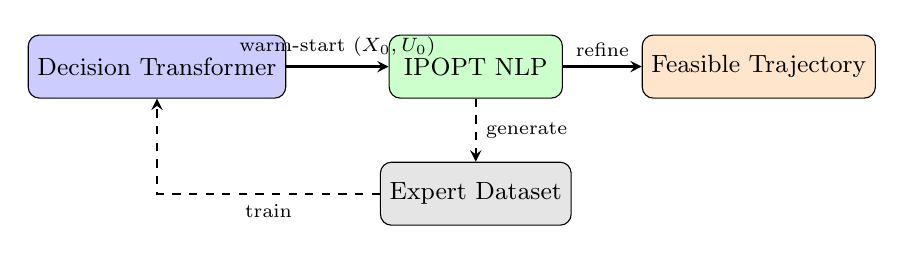
\begin{tikzpicture}[
    node distance=0.8cm,
    box/.style={rectangle, draw, rounded corners, minimum height=0.8cm, minimum width=2.2cm, text centered, font=\small},
    arrow/.style={->, >=stealth, thick}
]
\node[box, fill=blue!20] (dt) {Decision Transformer};
\node[box, fill=green!20, right=1.3cm of dt] (ipopt) {IPOPT NLP};
\node[box, fill=orange!20, right=1.0cm of ipopt] (out) {Feasible Trajectory};

\draw[arrow] (dt) -- node[above, font=\scriptsize] {warm-start $(X_0,U_0)$} (ipopt);
\draw[arrow] (ipopt) -- node[above, font=\scriptsize] {refine} (out);

\node[box, fill=gray!20, below=0.8cm of ipopt] (data) {Expert Dataset};
\draw[arrow, dashed] (ipopt) -- node[right, font=\scriptsize] {generate} (data);
\draw[arrow, dashed] (data) -| node[below, font=\scriptsize, pos=0.25] {train} (dt);
\end{tikzpicture}
\caption{Hybrid warm-starting pipeline. DT proposes a trajectory initialization; IPOPT enforces hard constraints and refines to a locally optimal solution.}
\label{fig:pipeline}
\end{center}
\vskip -0.2in
\end{figure}

\section{Approach}
\label{sec:approach}

\subsection{Vehicle model and minimum-time NLP}

The dynamics model follows the single-track formulations used in recent autonomous racing studies \cite{subositsgerdes2021fidelity,aggarwal2025friction}: left/right tires are lumped per axle, planar rigid-body dynamics are retained, and nonlinear tire forces are represented with a Fiala-style brush model. The trajectory is parameterized by arc length $s$ to align optimization constraints with track geometry. Let $k=0,\dots,N$ index spatial nodes with spacing $\Delta s$, and let decision variables be $\mathbf{X}=[\mathbf{x}_0,\dots,\mathbf{x}_N]$ and $\mathbf{U}=[\mathbf{u}_0,\dots,\mathbf{u}_N]$, with
\begin{equation}
\mathbf{x} = [u_x, u_y, r, \Delta F_{z,\text{long}}, \Delta F_{z,\text{lat}}, t, e, \Delta\psi]^\top,\quad
\mathbf{u} = [\delta, F_x]^\top.
\end{equation}
This state choice extends the standard $(u_x,u_y,r,t,e,\Delta\psi,\Delta F_z)$ representation by retaining both longitudinal and lateral load-transfer states used by the current simulator/optimizer implementation. Kinematic path relations follow the same structure as prior work:
\begin{equation}
\dot{s} = \frac{u_x\cos\Delta\psi-u_y\sin\Delta\psi}{1-\kappa(s)e},\qquad
\dot{e}=u_x\sin\Delta\psi+u_y\cos\Delta\psi,\qquad
\Delta\dot{\psi}=r-\kappa(s)\dot{s}.
\end{equation}
The NLP objective is minimum lap time with a lightweight control-smoothness regularizer:
\begin{equation}
\min_{\mathbf{X},\mathbf{U}} \; J
= t_N
+ \lambda_u \sum_{k=0}^{N-1}\|\mathbf{u}_{k+1}-\mathbf{u}_k\|_2^2.
\end{equation}
Dynamic continuity is enforced by trapezoidal collocation in spatial form, consistent with racing trajectory-optimization practice:
\begin{equation}
\mathbf{x}_{k+1} = \mathbf{x}_k + \frac{\Delta s}{2}
\left(
f_s(\mathbf{x}_k,\mathbf{u}_k) + f_s(\mathbf{x}_{k+1},\mathbf{u}_{k+1})
\right),
\end{equation}
where $f_s(\cdot)$ denotes the spatial-form dynamics $\dot{\mathbf{x}}/\dot{s}$, and the along-track rate $\dot{s}$ appears implicitly through the kinematics. The NLP includes hard track bounds, actuator limits, and two numerically critical constraints:
\begin{align}
\dot{s}_k &\ge \varepsilon_s \quad \text{(forward progress)},\\
1-\kappa(s_k)e_k &\ge \varepsilon_\kappa \quad \text{(Frenet non-singularity)}.
\end{align}
For full-lap solutions, periodic closure is imposed as $\mathbf{x}_0=\mathbf{x}_N$ and $\mathbf{u}_0=\mathbf{u}_N$ for all states/controls except time (with $t_0=0$ and $t_N$ free). The resulting sparse NLP is solved with IPOPT through CasADi, matching the solver stack commonly used in the cited vehicle-planning literature.

\subsection{Obstacle handling and acceptance-gated retries}

Static circular obstacles are enforced via node-based clearance constraints in the world frame:
\begin{equation}
\|p(s_k,e_k)-p_{\text{obs},i}\|_2^2 \ge (r_i + m_i + R_{\text{veh}} + c)^2,
\end{equation}
where $p(s,e)$ is the Frenet-to-ENU map, $r_i$ is obstacle radius, $m_i$ is a safety margin, $R_{\text{veh}}$ is an inflated vehicle footprint radius, and $c$ is an optional additional clearance. To avoid over-complicating the NLP early, obstacle constraints are kept simple in the optimizer, while safety is enforced with a dense post-solve collision check (sub-sampled along each segment). 

An \emph{acceptance-gated retry policy} is then applied: if IPOPT converges but violates dense clearance by more than a small tolerance, the same scenario is retried with higher discretization ($N$) and/or denser obstacle sampling. This produces reliable accepted expert demonstrations while also surfacing failure modes that DT warm-starting should reduce (e.g., converging quickly to a trajectory that ``cuts'' an obstacle).

\subsection{Dataset contract (expert trajectories)}

Each accepted solve is stored as an episode with:
(i) a reproducibility header (map identifier/hash, $N$, $\Delta s$, obstacle list, solver settings, seed),
(ii) per-step arrays $(s_k, \mathbf{x}_k, \mathbf{u}_k, \Delta t_k)$, and
(iii) derived features: global pose $(E_k,N_k,\psi_k)$, track curvature $\kappa(s_k)$, and RTG defined as $\mathrm{RTG}_k=-\sum_{j=k}^{N-1}\Delta t_j$.
Storing the full internal state (including load-transfer states) keeps the data future-proof even if DT only observes a subset.

\subsection{Decision Transformer warm-start (planned)}

DT will be trained as a causal decoder that predicts controls conditioned on RTG and a compact observation:
\begin{equation}
\mathbf{z}_k = [\mathrm{RTG}_k,\; \mathbf{o}_k,\; \mathbf{u}_{k-1}],
\end{equation}
where $\mathbf{o}_k$ includes $(u_x,u_y,r,e,\Delta\psi)$, local track features $(\kappa,\text{half-width})$, and a fixed-size obstacle tensor (e.g., the $M$ nearest obstacles within a lookahead window, represented in Frenet-relative coordinates). At inference, the DT-generated $(X_0,U_0)$ is passed directly to IPOPT as an initialization.

\section{Milestone progress and preliminary results}
\label{sec:results}

\textbf{Implemented.} The current codebase includes: a unified vehicle dynamics model; a spatial direct-collocation IPOPT optimizer; consistent Frenet-to-ENU mapping between optimization and visualization; a compiled solver path; and batch evaluation scripts that sample random obstacle scenarios and apply acceptance-gated retries.

\textbf{Early quantitative results.} On the Medium Oval map with $3$--$6$ randomly sampled obstacles per scenario, a batch of $20$ scenarios achieved $100\%$ IPOPT convergence and $100\%$ acceptance under the practical clearance gate $\min(\text{dense clearance})\ge -10^{-3}$\,m. However, a single baseline attempt (with fixed $N$ and obstacle subsampling) is accepted only 0.20 of the time; retries are frequently required to satisfy dense clearance.

Table~\ref{tab:batch} summarizes the batch statistics (selected attempt per scenario after retries), and contrasts them with the baseline attempt.

\begin{table}[t]
\caption{Batch evaluation on Medium Oval (20 scenarios, mean 5 obstacles). ``Baseline'' refers to the first solve attempt; ``Selected'' refers to the accepted attempt after retries (higher $N$ and/or denser obstacle sampling). Times/iterations reflect the recorded solver logs for this batch.}
\label{tab:batch}
\vskip 0.15in
\begin{center}
\begin{small}
\begin{tabular}{lcccc}
\toprule
Method & Accept rate & Time [s] (mean) & IPOPT iters (mean) & Cost [s] (mean)\\
\midrule
Baseline attempt & 0.20 & 17.7 & 37.0 & 24.57 \\
Selected (after retries) & 1.00 & 21.6 & 32.6 & 24.05 \\
\bottomrule
\end{tabular}
\end{small}
\end{center}
\vskip -0.1in
\end{table}

The selected attempts used the following retry outcomes: baseline accepted in 4/20 scenarios, higher-$N$ accepted in 7/20, and higher obstacle subsampling accepted in 9/20. These statistics motivate DT warm-starting as a way to (i) reduce the need for retries and (ii) reduce the interior-point iterations required to reach a safe local optimum.

\begin{figure}[t]
\vskip 0.1in
\begin{center}
\IfFileExists{results/trajectory_optimization/ipopt_single_stage_trajectory.png}{
\centerline{\includegraphics[width=\columnwidth]{results/trajectory_optimization/ipopt_single_stage_trajectory.png}}
}{
\IfFileExists{fig_trajectory.png}{
\centerline{\includegraphics[width=\columnwidth]{fig_trajectory.png}}
}{
\fbox{\parbox{0.95\columnwidth}{\vspace{0.4cm}\centering Trajectory figure not found.\vspace{0.4cm}}}
}
}
\caption{Representative IPOPT solution on the oval track with obstacles (current pipeline output).}
\label{fig:solver_output}
\end{center}
\vskip -0.2in
\end{figure}

\textbf{Observed limitations.} Some adversarial obstacle placements still yield converged but unsafe trajectories (significant negative dense clearance) even after retries, indicating that (a) the current obstacle constraint discretization may be too coarse in extreme scenes, and (b) the initializer and/or constraint enforcement needs strengthening before large-scale dataset generation.

\section{Remaining work}
\label{sec:remaining}

\textbf{Expert/data pipeline (near-term).}
(1) Finalize the Tier-1 solver settings and obstacle inflation so that acceptance-gated retries succeed on a broader set of obstacle scenes; 
(2) implement the canonical dataset schema and generate a sufficiently large set of accepted trajectories (obstacle-free base laps, then randomized obstacle layouts via a curriculum on obstacle count and size).

\textbf{DT training and integration.}
(3) Train the Decision Transformer on RTG-conditioned sequences with track and obstacle features; 
(4) integrate DT outputs as IPOPT warm-start initializations $(X_0,U_0)$.

\textbf{Evaluation (final milestone).}
(5) Compare DT-warm-start vs.\ baseline initialization on: (i) IPOPT iterations, (ii) wall-clock solve time, (iii) acceptance rate without retries, and (iv) final lap time / constraint margins. Additional ablations will vary context length and obstacle feature sets to understand which information drives warm-start quality.

\bibliography{example_paper}
\bibliographystyle{icml2018}

\end{document}
